\documentclass[
	10pt,								% globale Schriftgröße
	parskip=half-,						% setzt Absatzabstand hoch
	paper=a4,							% Format
	english,ngerman,					% lädt Sprachpakete
	]{scrartcl}							% Dokumentenklasse

% //////////////////// Pakete laden ////////////////////
\usepackage{amsmath}			% MUSS vor fontspec geladen werden
\usepackage{mathtools}			% modifiziert amsmath
\usepackage{amssymb}			% mathematische symbole, für \ceckmarks
\usepackage{amsthm}				% für proof
\usepackage{mathrsfs}			% für \mathscr
\usepackage{latexsym}
\usepackage{marvosym}				% für Lightning

\usepackage{fontspec} 			% funktioniert nur mit den neueren Compilern z.B. XeLaTeX
\usepackage{microtype}			% für bessere Worttrennung
\usepackage[ngerman]{babel} 	% Spracheinstellung
\usepackage{lmodern}			% verändert verwendete Schriftart, damit sie weniger pixelig ist

\usepackage{verbatim}
\usepackage{listings}			% Für Quellcode

\usepackage{graphicx}
\usepackage{tabularx}			% für Tabellen mit gleicher Spaltenbreite und automatischen Umbrüchen
\usepackage{fullpage}
\usepackage{multirow}			% für multirow in tabulars
\usepackage{rotate}
\usepackage[cmyk,table]{xcolor} % um Farben zu benutzen, kann mehr als das Paket color
\usepackage[					% Verlinkungen
	colorlinks,					% farbige Schrift, statt farbiger Rahmen
	linktocpage,				% verlinkt im Abb.Verzeichnis Seitenzahl statt Bildunterschrift
	linkcolor=blue				% setzt Farbe der Links auf blau
	]{hyperref}					% nur für digitale Anwendungen, url = "http://www.example.com"
\usepackage{url}				% für Webadressen wie e-mail usw.: "\url{http://www.example.com}"

\usepackage{enumerate}			% für versch. Aufzählungezeichen wie z.B. a)
\usepackage{xspace}				% folgt ein Leerzeichen nach einem \Befehl, wird es nicht verschluckt.
\usepackage{cancel}				% für das Durchstreichen u.a. in Matheformeln mit \cancel
\usepackage{float}              % zum Forcieren der Position von figure-Umgebungen

% zum Zeichnen (u.a. von Graphen)
\usepackage{fp}
\usepackage{tikz}
\usetikzlibrary{tikzmark}			% für \tikzmark{toRemember}
\usetikzlibrary{positioning}	% verbesserte Positionierung der Knoten
\usetikzlibrary{automata}		% für Automaten (GTI)
\usetikzlibrary{arrows}
\usetikzlibrary{shapes}
\usetikzlibrary{decorations.pathmorphing}
\usetikzlibrary{decorations.pathreplacing}
\usetikzlibrary{decorations.shapes}
\usetikzlibrary{decorations.text}

% //////////////////// Syntaxhighlighting ////////////////////
\lstloadlanguages{Python, Haskell, [LaTeX]TeX, Java}
\lstset{
   basicstyle=\footnotesize\ttfamily,	% \scriptsize the size of the fonts that are used for the code
   backgroundcolor = \color{bgcolour},	% legt Farbe der Box fest
   breakatwhitespace=false,	% sets if automatic breaks should only happen at whitespace
   breaklines=true,			% sets automatic line breaking
   captionpos=t,				% sets the caption-position to bottom, t for top
   commentstyle=\color{codeblue}\ttfamily,% comment style
   frame=single,				% adds a frame around the code
   keepspaces=true,			% keeps spaces in text, useful for keeping indentation
							% of code (possibly needs columns=flexible)
   keywordstyle=\bfseries\ttfamily\color{codepurple},% keyword style
   numbers=left,				% where to put the line-numbers;
   							% possible values are (none, left, right)
   numberstyle=\tiny\color{codegreen},	% the style that is used for the line-numbers
   numbersep=5pt,			% how far the line-numbers are from the code
   stepnumber=1,				% nummeriert nur jede i-te Zeile
   showspaces=false,			% show spaces everywhere adding particular underscores;
							% it overrides 'showstringspaces'
   showstringspaces=false,	% underline spaces within strings only
   showtabs=false,			% show tabs within strings adding particular underscores
   flexiblecolumns=false,
   tabsize=1,				% the step between two line-numbers. If 1: each line will be numbered
   stringstyle=\color{orange}\ttfamily,	% string literal style
   numberblanklines=false,				% leere Zeilen werden nicht mitnummeriert
   xleftmargin=1.2em,					% Abstand zum linken Layoutrand
   xrightmargin=0.4em,					% Abstand zum rechten Layoutrand
   aboveskip=2ex, 
}

\lstdefinestyle{py}{
   language=Python,
}
\lstdefinestyle{hs}{
   language=Haskell,
}
\lstdefinestyle{tex}{
	language=[LaTeX]TeX,
	escapeinside={\%*}{*)},     % if you want to add LaTeX within your code
	texcsstyle=*\bfseries\color{blue},% hervorhebung der tex-Schlüsselwörter
	morekeywords={*,$,\{,\},\[,\],lstinputlisting,includegraphics,
	rowcolor,columncolor,listoffigures,lstlistoflistings,
	subsection,subsubsection,textcolor,tableofcontents,colorbox,
	fcolorbox,definecolor,cellcolor,url,linktocpage,subtitle,
	subject,maketitle,usetikzlibrary,node,path,addbibresource,
	printbibliography},% if you want to add more keywords to the set
     numbers=none,
     numbersep=0pt,
     xleftmargin=0.4em,
}

\lstdefinestyle{java}{
	language=Java,
	extendedchars=true,		% lets you use non-ASCII characters;
   						% for 8-bits encodings only, does not work with UTF-8
}

\lstdefinelanguage[x64]{Assembler}     % add a "x64" dialect of Assembler
   [x86masm]{Assembler} % based on the "x86masm" dialect
   % with these extra keywords:
   {morekeywords={CDQE,CQO,CMPSQ,CMPXCHG16B,JRCXZ,LODSQ,MOVSXD, %
                  POPFQ,PUSHFQ,SCASQ,STOSQ,IRETQ,RDTSCP,SWAPGS, %
                  rax,rdx,rcx,rbx,rsi,rdi,rsp,rbp, %
                  r8,r8d,r8w,r8b,r9,r9d,r9w,r9b}
}					% for 8-bits encodings only, does not work with UTF-8

\lstdefinestyle{c}{
	language=c,
	extendedchars=true,		% for 8-bits encodings only, does not work with UTF-8
}

% //////////////////// eigene Kommandos ////////////////////
\newcommand\FU{Freie Universität Berlin\xspace}% benötigt package xspace
\newcommand\gdw{g.\,d.\,w.\xspace}
\newcommand\oBdA{o.\,B.\,d.\,A.\xspace}
\newcommand{\Eu}{\texteuro}
\newcommand\N{\mathbb{N}\xspace}
\newcommand\Q{\mathbb{Q}\xspace}
\newcommand\R{\mathbb{R}\xspace}
\newcommand\Z{\mathbb{Z}\xspace}
\newcommand\ohneNull{\ensuremath{\backslash\lbrace 0\rbrace}}% \{0}
\let\dhALT\dh	% Schreibt Befehl \dh in \dhALT um
\renewcommand\dh{d.\,h.\xspace}	%renew überschreibt command \dh
\newcommand\Bolt{\;\text{\LARGE\raisebox{-0.3em}{\Lightning}\normalsize}\xspace}% Blitz
\newcommand\zz{\ensuremath{\raisebox{+0.25ex}{Z}% zu zeigen
			\kern-0.4em\raisebox{-0.25ex}{Z}%
			\;\xspace}}
\newcommand{\from}{\ensuremath{\colon}}
\newcommand{\floor}[1]{\lfloor{#1}\rfloor}
\newcommand{\ceil}[1]{\lceil{#1}\rceil}
 \renewcommand{\L}{\ensuremath{\mathcal{L}}\xspace}
 \renewcommand{\P}{\ensuremath{\mathcal{P}}\xspace}
 \newcommand{\NL}{\ensuremath{\mathcal{N}\kern-0.2em\mathcal{L}}\xspace}
 \newcommand{\NP}{\ensuremath{\mathcal{NP}}\xspace}

% //////////////////// Mathefunktionen ////////////////////
\DeclareMathOperator{\Landau}{\mathcal{O}}
\DeclareMathOperator{\True}{True}
\DeclareMathOperator{\False}{False}

% //////////////////// eigene Theoreme ////////////////////
\newtheorem{theorem}{Satz}
\newtheorem{corollary}[theorem]{Folgerung}
\newtheorem{lemma}[theorem]{Lemma}
\newtheorem{observation}[theorem]{Beobachtung}
\newtheorem{definition}[theorem]{Definition}
\newtheorem{Literatur}[theorem]{Literatur}
% konfiguriert proof
\makeatletter
\newenvironment{Proof}[1][\proofname]{\par
  \pushQED{\qed}%
  \normalfont \topsep6\p@\@plus6\p@\relax
  \trivlist
  \item[\hskip\labelsep
%         \itshape
        \bfseries
    #1\@addpunct{.}]\ignorespaces
}{%
  \popQED\endtrivlist\@endpefalse
}
\makeatother

% //////////////////// eigene Farben ////////////////////
\let\definecolor=\xdefinecolor
\definecolor{FUgreen}{RGB}{153,204,0}
\definecolor{FUblue}{RGB}{0,51,102}

\definecolor{middlegray}{rgb}{0.5,0.5,0.5}
\definecolor{lightgray}{rgb}{0.8,0.8,0.8}
\definecolor{orange}{rgb}{0.8,0.3,0.3}
\definecolor{azur}{rgb}{0,0.7,1}
\definecolor{yac}{rgb}{0.6,0.6,0.1}
\definecolor{Pink}{rgb}{1,0,0.6}

\definecolor{bgcolour}{rgb}{0.97,0.97,0.97}
\definecolor{codegreen}{rgb}{0,0.6,0}
\definecolor{codegray}{rgb}{0.35,0.35,0.35}
\definecolor{codepurple}{rgb}{0.58,0,0.82}
\definecolor{codeblue}{rgb}{0.4,0.5,1}

% //////////////////// eigene Settings ////////////////////

\textheight = 230mm		% Höhe des Satzspiegels / Layouts
\footskip = 10ex			% Abstand zw. Fußzeile und Grundlinie letzter Textzeile
\parindent 0pt			% verhindert Einrückung der 1. Zeile eines Absatzes
\setkomafont{sectioning}{\rmfamily\bfseries}% setzt Ü-Schriften in Serifen, {disposition}

\newcommand{\dozent}{Lutz Prechelt}
\newcommand{\tutor}{Samuel Domiks}
\newcommand{\tutoriumNo}{02\\Materialien: Latex, Skript}
\newcommand{\ubungNo}{09}
\newcommand{\veranstaltung}{Softwaretechnik}
\newcommand{\semester}{SoSe21}
\newcommand{\studenten}{Jonny Lam \& Thore Brehmer}

% /////////////////////// BEGIN DOKUMENT /////////////////////////
\begin{document}
% /////////////////////// BEGIN TITLEPAGE /////////////////////////
\begin{titlepage}
	\subject{\dozent}
	\title{\veranstaltung, \semester}
	\subtitle{\Large Übung \ubungNo\\ \large\vspace{1ex} TutorIn: \tutor\\ Tutorium \tutoriumNo}
	\author{\studenten}
	\date{\normalsize \today}
\end{titlepage}

\maketitle								% Erstellt das Titelblatt
\vspace*{-10cm}							% rückt Logo an den oberen Seitenrand
\makebox[\dimexpr\textwidth+1cm][r]{	%rechtsbündig und geht rechts 1cm über Layout hinaus
	
\includegraphics[width=0.4\textwidth]{src/fu_logo} % fügt FU-Logo ein
}
% /////////////////////// END TITLEPAGE /////////////////////////

\vspace{7cm}							% Abstand
\rule{\linewidth}{0.8pt}				% horizontale Linie

% /////////////////////// Task 1 /////////////////////////
\section{Begriffe}
\begin{enumerate}[(a)]
    % /////////////////////// a /////////////////////////
    \item {\itshape Was versteht man im Kontext der Softwareentwicklung unter dem Begriff „Information Hiding“ ? Erläutern Sie das Prinzip und erklären Sie, in welchem Zusammenhang es zum „Need to Know“-Prinzip steht.} \\
    Unter „Information Hiding" versteht man, das verstecken/verbergen von Daten und Informationen vor anderen Zugriffen bzw. vom Zugriff von außen.\\
    Beim Need-to-know Prinzip verbirgt man die Informationen um Risiken in  Vorhinein zu reduzieren.\\ Die Informationen sind nur für die, die es brauchen zugänglich.[1]
    % /////////////////////// b /////////////////////////
    \item {\itshape Warum ist das Prinzip des Information Hiding sinnvoll? Erläutern Sie dieses an einem Beispiel.} 
    Angenommen wir entwickeln ein Programm um das Gehalt der Mitarbeiter zu berechnen.\\ Dann will ich nicht, dass meine Mitarbeiter freien Zugang zu der Methode haben, die den Gehalt berechnet.\\ Zum einen, weil die sich beschweren können warum der andere mehr bekommt oder auch, dass Konkurrenten (andere Arbeitgeber) mehr bieten können. Also Information Hiding ist sinnvoll um wichtige Informationen vor Personen zu schützen, denen das nichts angeht bzw. von dem man nicht will, dass sie die Information bekommen.
   

    % /////////////////////// c /////////////////////////
    \item {\itshape Was versteht man unter dem „Design by Contract“-Prinzip? In welchem Kontext wirdes eingesetzt und warum?} \\
    Durch Contracts (Verträge) werden Abmachungen zwischen einzelne Programmmodule (Aufrufender und Aufgerufener) gemacht für die Verwendung von Schnittstellen. Diese Verträge soll die Kommunikation zwischen Programmodule sicherstellen. [2]
   
    % /////////////////////// d /////////////////////////
    \item {\itshape Erläutern Sie, in welchem Zusammenhang die BegriffeOCL, Invariante, Design by Con-tract, precondition, constraints, postcondition stehen.} \\
    Mit \textbf{OCL} können wir bei der Modellierung notwendige Randbedingungen formell festlegen. 
    Diese Randbedingungen nennen wir auch \textbf{Constraints}, die nach dem „\textbf{Design by Contract}" Prinzip gehen. Von den Constraints gibt es mehrere Arten, einmal Invarianten, die sind zu jedem Zeitpunkt wahr. Dann gibt es noch \textbf{precondition} und \textbf{postcondition}, pre Condition muss vor dem Aufruf wahr sein und post Condition nach dem Aufruf. [3] \\
    \\
    \textbf{Quellen:}\\
    \textbf{[1]:} Vorlesung 13 und \url{https://de.wikipedia.org/wiki/Datenkapselung_(Programmierung)} \\
    \textbf{[2]:} Vorlesung 13 und \url{https://de.wikipedia.org/wiki/Design_by_contract} \\
    \textbf{[3]:} Vorlesung 13 und \url{https://de.wikipedia.org/wiki/Object_Constraint_Language#:~:text=Die%20Object%20Constraint%20Language%20(OCL,von%20Computerprogrammen%20formal%20festlegen%20können.&text=OCL%20ist%20seit%20der%20UML,besteht%20auch%20in%20der%20Modelltransformation.} \\
    
\end{enumerate}

% /////////////////////// Task 2 /////////////////////////
\section{OCL lesen und schreiben}
In einem Prüfungsverwaltungssystem sollen die Klausurergebnisse und die Punktzahlen derStudierenden bei den Lösungen der einzelnen Aufgaben verwaltet werden. Das folgende UML-Klassendiagramm modelliert einen Teil der benötigten Daten.

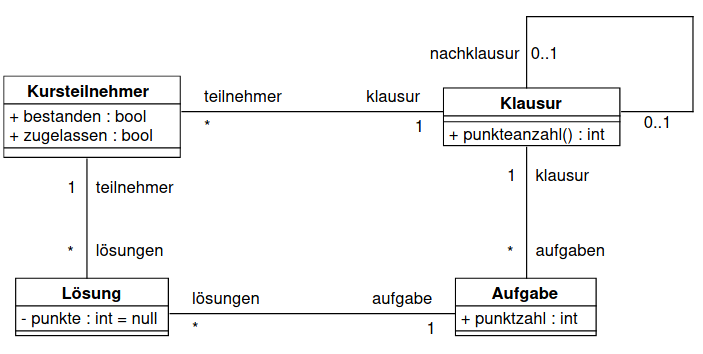
\includegraphics[width=1\textwidth]{src/u9/task2/uml.png}

    
\begin{enumerate}[(a)]
    % /////////////////////// a /////////////////////////
    \item {\itshape Drücken Sie auf Basis des Diagramms die OCL-Constraints c1 bis c3n natürlichsprachlich  aus,  also  in  einer  Form,  die  Sie  in  einem  Gespräch  mit  einer  Person  ohne Informatik-Hintergrund verwenden würden.}
    
    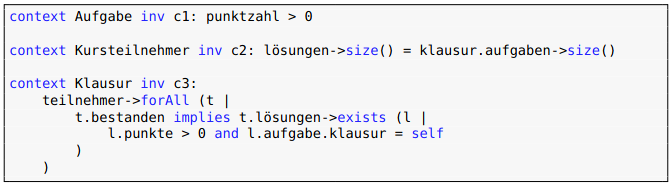
\includegraphics[width=1\textwidth]{src/u9/task2/code.png}
    
    \begin{enumerate}[{c}1:]
        \item Eine Aufgabe hat eine Punktzahl größer Null.
        \item Ein Kursteilnehmer hat genau soviel Lösungen, wie eine Klausur aufgaben hat. Anders gesagt: ein Kursteilnehmer muss genau eine Lösung für jede Klausur Aufgabe haben.
        \item Für jeden Teilnehmer an der Klausur gilt: Wenn die Klausur bestanden ist, dann hat jede Klausur Aufgabe von den Teilnehmer mehr als Null Punkte. Außerdem ist wichtig, dass die Aufgaben nicht Klausur übergreifend betrachtet werden. (Bsp. Klausur1: 1. bestanden, 2. nicht bestanden. Klausur2: 1. nicht bestanden, 2. bestanden.
        Daraus folgt trotzdem nicht bestanden!)
    \end{enumerate}
    
    % /////////////////////// b /////////////////////////
    \item {\itshape Geben Sie OCL-Constraints an, die die folgenden Sachverhalte formalisieren. AchtenSie darauf, syntaktisch einwandfreie OCL-Ausdrücke zu formulieren. Das schließt auchdie Beachtung der genauen Schreibweisen von Klassen, Attributen, Operationen undAssoziationen aus dem UML-Klassendiagramm ein.Schauen Sie auch in der OCL 2.4 Spezifikation (http://www.omg.org/spec/OCL/2.4/PDF) nach, falls Ihnen Ausdrucksmittel fehlen.}
    \begin{enumerate}
        \item {\itshape In jeder Klausur gibt es mindestens eine Aufgabe mit genau einem Punkt.}
        \lstinputlisting[language=python, linerange={1-3}]{src/u9/task2/ocl.txt}
        
        \item {\itshape Eine Nachklausur kann keine Nachklausur haben.}
        \lstinputlisting[language=python, linerange={5-8}]{src/u9/task2/ocl.txt}
        
        \item {\itshape Ist ein/e Kursteilnehmer/in zugelassen, gibt es für jede Klausuraufgabe auch eine Lösung von ihm/ihr.}
        \lstinputlisting[language=python, linerange={10-13}]{src/u9/task2/ocl.txt}

    \end{enumerate}

\end{enumerate}



% /////////////////////// Task 3 /////////////////////////
\section{OCL-Modellerweiterungen}
Diese Aufgabe baut auf dem gleichen UML-Modell auf wie Aufgabe 9-2. Nun soll zusätzlich auch die Klausurkorrektur modelliert werden: Bei der Korrektur geht der/die Dozent/in alle Lösungen einzeln durch, bewertet sie jeweils und errechnet die Gesamtpunktzahl für jede/n Teilnehmer/in.

    
\begin{enumerate}[(a)]
    % /////////////////////// a /////////////////////////
    \item {\itshape Erweitern Sie das Modell nun um eine Operation korrigieren mit passender Signatur sowie  ein  neues  Attribut;  darüber  hinaus  darf das  Klassendiagramm  in  keiner  Weise verändert werden (also keine neuen Klassen, veränderte Sichtbarkeiten, etc.). Die Operation korrigieren wird aufgerufen, sobald der/die Dozent/in eine Lösung korrigiert hat.
    Es soll damit insbesondere möglich sein, dass
    \begin{itemize}
        \item das Attribut punkte in Lösung gefüllt wird, und
        \item die erreichte Gesamtpunktzahl des Teilnehmers aktualisiert wird.
    \end{itemize}
    Beschreiben Sie zunächst verbal, was korrigieren genau leisten soll. Finden Sie geeignete  Stellen  (und  für  das  neue  Attribut:  auch  einen  geeigneten  Namen)  für  die neuen Member im Klassendiagramm.
    }
    
    \textbf{Lösung:}
    \begin{itemize}
        \item Die Methode korrigieren soll punkte in den Lösungen sowie in der Gesamtpunktzahl des Teilnehmers aktualisieren. 
        \item Da die punkte von Lösungen privat sind, wir aber darauf zugriff brauchen, schreiben wir die \underline{Methode in die Klasse Lösung}. Also: \textbf{+korrigieren(punkte: int)}
        \item Damit wir die Gesamtpunktzahl für den Kursteilnehmer eintragen können, erstellen wir ein public Attribut \underline{gesamtpunktanzahl im Kursteilnehmer}. Also: \textbf{+gesamtpunktanzahl : int}
    \end{itemize}
    
    % /////////////////////// b /////////////////////////
    \item {\itshape Gehen Sie zunächst in einer ersten Version davon aus, dass korrigieren nur einmal pro Exemplar der Klasse Lösung aufgerufen werden darf; die einmal gesetzte Punktzahl ist danach unveränderlich. Spezifizieren Sie sowohl möglichst strenge Vorbedingungen für Ihre Operation korrigieren, als auch alle Effekte(post condition)der Operation komplett in OCL.}
    
    Wir möchten mit den OCL Bedienungen folgendes aussagen:
    \begin{itemize}
        \item \textbf{Pre:}
        \begin{itemize}
            \item Es können nur Lösungen korrigiert werden, welche noch nicht korrigiert wurden.
            \item Es dürfen nicht negative Punkte für die Lösung eingetragen werden.
            \item Es dürfen nicht mehr Punkte, als die Aufgabe angibt, für die Lösung eingetragen werden.
            \item Der Teilnehmer muss zugelassen sein, damit eine Lösung korrigiert wird.
        \end{itemize}
        
        \item \textbf{Post:}
        \begin{itemize}
            \item Nach der Korrektur wurden die Punkte korrekt eingetragen.
            \item Nach der Korrektur wurde die Lösung wirklich korrigiert (Vielleicht unnötig?)
            \item Nach der Korrektur wurden die Punkte auf die Gesamtpunktzahl des Teilnehmers addiert.
        \end{itemize}
        
    \lstinputlisting[language=python, linerange={1-12}]{src/u9/task3/ocl3.txt}
    \end{itemize}



    % /////////////////////// c /////////////////////////
    \item {\itshape Gehen Sie nun von der realistischeren Anforderung aus, dasskorrigierenmehrfachaufgerufen werden kann, um z.B. die Punktzahl einer Lösung bei einer Klausureinsichtzu korrigieren.Spezifizieren  Sie  wiederum  möglichst  strenge  Vorbedingungen  und  alle  Effekte  derOperation in OCL.}
    \begin{itemize}
        \item Wir haben lediglich die Bedienung \dq Es können nur Lösungen korrigiert werden, welche noch nicht korrigiert wurden.\dq \ aus Zeile 4 entfernt.
        \item Sowie zu der Bedienung \dq Nach der Korrektur wurden die Punkte auf die Gesamtpunktzahl des Teilnehmers addiert.\dq \ aus Zeile 12 (jetzt 11) etwas hinzugefügt.
        \item Denn nun muss der alte Punkte Wert für die Aufgabe noch von der Gesamtpunktzahl abgezogen werden, wenn man einen neuen Punkte Wert hinzu addiert will.
    \end{itemize}
    \lstinputlisting[language=python, linerange={15-25}]{src/u9/task3/ocl3.txt}

    % /////////////////////// d /////////////////////////
    \item {\itshape Spezifizieren Sie den Effekt der OperationKlausur.punkteanzahlunter Verwendungdes OCL-Schlüsselwortesresult.Hinweis: Der resultierende Ausdruck passt bequem auf eine Zeile. Recherchieren Siebei Bedarf nach OCL-Collections und ihren Operationen.}
    \lstinputlisting[language=python, linerange={28-30}]{src/u9/task3/ocl3.txt}

\end{enumerate}




\end{document}